% !TEX root = ../msimplicial.tex

\section{Multisimplicial algebraic topology} \label{s:multisimplicial}

\subsection{Multisimplicial sets} \label{ss:multisimplicial sets}

Let us consider an arbitrary positive integer~$k$.
The \textit{$k$-fold multisimplex category} $\simplex^{\times k}$ is the $k$-fold Cartesian product of the simplex category $\simplex$.
The category
\[
\mSet{k} \defeq \Fun\big((\simplex^{\times k})^\op, \Set\big)
\]
is referred to as the category of \textit{$k$-fold multisimplicial sets}.
We remark that $\mSet{1}$ and $\mSet{2}$ are naturally equivalent to the categories of simplicial and bisimplicial sets respectively.
The representable $k$-fold multisimplicial sets are denoted by
\[
\simplex^{n_1,\dots,n_k} \defeq
\yoneda \big([n_1]\times\dots\times[n_k]\big),
\]
and there are canonical bijections
\[
\simplex^{n_1,\dots,n_k} \big([m_1]\times\dots\times[m_k]\big) \cong
\simplex^{n_1}_{m_1}\times\dots\times\simplex^{n_k}_{m_k}.
\]

Explicitly, a $k$-fold multisimplicial set $X$ consists of a collection of sets
\[
X_{m_1,\dots,m_k} =
X \big( [m_1] \times\dots\times [m_k] \big)
\]
indexed by tuples of non-negative integers $(m_1,\dots,m_k)$ together with \textit{face maps}
\[
\face_i^j \colon
X_{m_1, \dots, m_j,\dots,m_k} \to
X_{m_1, \dots, m_j-1, \dots, m_k}
\]
and \textit{degeneracy map}
\[
\dege^j_i \colon X_{m_1, \dots, m_j,\dots,m_k} \to X_{m_1, \dots, m_j+1, \dots, m_k}
\]
for $1 \leq j \leq k$ and $0 \leq i \leq m_j$ such that, referring to $j$ as the \textit{direction} of these maps, two of them satisfy the simplicial identities when they have the same direction and commute when they do not.
An element of $X_{m_1,\dots,m_k}$ is called
$(m_1,\dots,m_k)$-\textit{multisimplex}.
A multisimplex is \textit{degenerate} if it is in the image of a degeneracy map.

\subsection{Geometric realization} \label{ss:geometric realization}

We will use the following model of the topological simplex:
\[
\gsimplex^n = \big\{
(t_1, \dots, t_n) \in [0,1]^n \mid t_1 \geq \dots \geq t_n
\big\}
\]
with
\[
\delta_i(t_1, \dots, t_n) =
\begin{cases}
	(1, t_1, \dots, t_n) & i = 0, \\
	(t_1, \dots, t_i, t_i, \dots, t_n) & 0 < i < n, \\
	(t_1, \dots, t_n, 0) & i = n,
\end{cases}
\]
and
\[
\sigma_i(t_1, \dots, t_n) = (t_1, \dots, \widehat t_i, \dots, t_n).
\]

The \textit{geometric realization} functor
\[
\bars{-} \colon \mSet{k} \to \Top
\]
is the Yoneda extension of the functor defined on representable objects by
\[
\bars{\simplex^{n_1,\dots,n_k}} \defeq
\gmsimplex{n_1}{n_k}.
\]
Explicitly, for a $k$-fold multisimplicial set $X$ we have
\begin{align*}
	\bars{X} &\cong
%	\colim_{\cramped{(\simplex^{n_1,\dots,n_k} \downarrow X})} \, \bars{\simplex^{n_1,\dots,n_k}} \\ &=
	\coprod \gmsimplex{n_1}{n_k} \times X_{n_1,\dots,n_k} /_\sim
\end{align*}
where
\[
\begin{split}
	(V_1, \dots, V_j, \dots, V_k, \face^j_i(x)) &\sim (V_1, \dots, \delta_i(V_j), \dots, V_k, x), \\
	(V_1, \dots, V_j, \dots, V_k, \dege^j_i(x)) &\sim (V_1, \dots, \sigma_i(V_j), \dots, V_k, x), \todo{@paolo: I don't think this is right. Is $t_i$ a real number? It seems its a vector.@anibal these are vectors I changed notation}
\end{split}
\]
which equips $\bars{X}$ with a canonical cellular structure.

The geometric realization functor has a right adjoint
\[
\Sing^{(k)} \colon \Top \to \mSet{k}
\]
defined on a topological space $\fZ$, as usual, by the expression
\[
\Sing^{(k)}(\fZ)_{n_1,\dots,n_k} \defeq
\Top(\gmsimplex{n_1}{n_k},\fZ).
\]

These define a Quillen equivalence. \todo{@anyone: a reference to the bisimplicial Quillen equivalence proof would be good}

\subsection{Algebraic realization} \label{ss:algebraic realization}

The functor of \textit{chains}
\[
\chains \colon \mSet{k} \to \Ch,
\]
is the Yoneda extension of the functor defined on representable objects by
\[
\chains \big( \simplex^{n_1, \dots, n_k} \big) \defeq
\chains(\simplex^{n_1}) \ot \dotsb \ot \chains(\simplex^{n_k}).
\]
It is naturally isomorphic to the composition of the geometric realization functor and the functor of cellular chains with respect to the canonical cellular structure.

Explicitly, for a $k$-fold multisimplicial set $X$ the $\k$-module $\chains(X)_n$ is freely generated by the non-degenerate $(n_1, \dots, n_k)$-multisimplices $x$ with $n_1+\dots+n_k = n$ and differential given by
\[
d(x) = \sum_{j=1}^k \sum_{\ell_j=1}^{n_j}
(-1)^{n_{1}+\dots+n_{j-1}+\ell_j} \, d^j_{\ell_j}(x).
\]

%\begin{remark*}
%	If we do not mod out by degenerate multisimplices the same formula defines the functor of \textit{non-normalized chains}.
%	A slight generalization of the classical normalization theorem by MacLane \cite{MacLane} shows that the natural projection between these is a natural chain homotopy equivalence. \todo{@andrea: please get the missing reference.}
%\end{remark*}

For any topological space $\fZ$ the complex of chains of $\Sing^{(k)}(\fZ)$ is denoted $\rS^{(k)}(\fZ)$ and referred to as the $k$-\textit{fold singular chains} of $\fZ$.

\subsection{Coalgebra structure} \label{ss:coalgebra}

A \textit{counital coalgebra} structure on a chain complex $C$ is a pair of chain maps $\copr \colon C \to C \ot C$ and $\aug \colon C \to \k$ satisfying
\[
(\id \ot \aug) \circ \copr =
\id =
(\aug \ot\, \id) \circ \copr.
\]
For each $n \in \N$, the complex $\chains(\simplex^n)$ is naturally equipped with a counital coalgebra structure defined by:
\[
\begin{split}
	\copr \big( [v_0, \dots, v_m] \big) &=
	\sum_{i=0}^m \, [v_0, \dots, v_i] \ot [v_i, \dots, v_m], \\
	\aug \big( [v_0, \dots, v_q] \big) &=
	\begin{cases} 1 & \text{ if } q = 0, \\ 0 & \text{ if } q>0. \end{cases}
\end{split}
\]

The tensor product of two counital coalgebras $C$ and $C'$ is one too with structure maps given by:
\begin{gather*}
	C \ot C^\prime \xra{\copr \ot \copr^\prime}
	(C \ot C) \ot (C^\prime \ot C^\prime) \xra{(23)}
	(C \ot C^\prime) \ot (C \ot C^\prime), \\
	C \ot C^\prime \xra{\aug \ot \aug^\prime}
	\k \ot \k \xra{\cong} \k.
\end{gather*}

From these constructions we deduce a natural counital coalgebra structure on the chains of representable multisimplicial sets $\chains \big( \simplex^{n_1, \dots, n_k} \big) = \chains(\simplex^{n_1}) \ot \dotsb \ot \chains(\simplex^{n_k})$, and, via a Yoneda extension, one on the chains of general multisimplicial sets.
Explicitly, for a $k$-fold multisimplicial set $X$ and $(m_1,\dots,m_k)$-multisimplex $x$ let
\[
\fI_{m_1,\dots,m_k} = \set[\big]{(i_{1},\dots,i_{k}) \mid 0 \le i_j \le m_j,\ \forall j = 1,\dots,k},
\]
then
\[
\copr(x) =
\sum_{I\in \mathfrak{I}_{k,x}} \;
(-1)^{\sum_{1 \leq l<h \leq k} i_h (m_l-i_l) } \
x \rfloor_{(i_{1},\dots,i_{k})} \ot
\!\,_{(m_{1}-i_{1}, \dots, m_{k}-i_{k})} \lfloor x
\]
where the \textit{front $(i_1,\dots,i_k)$-face} of $x$ is the multisimplex
\[
x \rfloor_{(i_{1}, \dots, i_{k})} =
X(F_{i_1}, \dots, F_{i_k})(x) \in X_{i_1,\dots,i_k}
\]
with
$F_{i_j} \colon [i_j] \to [n_j]$ defined by $F_{i_j}(h)=h$, and the \textit{back $(i_1,\dots,i_k)$-face} of $x$ is the multisimplex
\[
\,_{(i_{1}, \dots, i_{k})} \lfloor x =
X(B_{i_1}, \dots, B_{i_k})(x) \in X_{i_1,\dots,i_k}
\]
with $B_{i_j} \colon [i_j] \to [n_j]$ defined by $B_j(h) = h+m_j-i_j$.

\subsection{\pdfEinfty-extension} \label{ss:e-infty extension}

An \textit{$\cM$-bialgebra} structure on counital coalgebra $(C, \copr, \aug)$ is a degree $1$ linear map $\pr \colon C \ot C \to C$ satisfying
%whose boundary is $(\aug \ot \, \id) - (\id \ot \aug)$, i.e.,
\[
\bd (c_1 \ast c_2) - \bd c_1 \ast c_2 + (-1)^{\bars{c_1}} c_1 \ast \bd c_2 =
\aug(c_1) c_2 - \aug(c_2) c_1,
\]
\[
\aug (c_1 \pr c_2) = 0.
\]
for all $c_1, c_2 \in C$.
As proven in \cite{medina2020prop1}, the collection of all maps $\set{C \to C^{\ot r}}_{r \in \N}$ generated by $\copr$, $\aug$ and $\pr$ make $C$ into an $E_\infty$-coalgebra, that is to say, a coalgebra over certain operad $\UM$ that is a cofibrant resolution of the terminal operad.

For any integer $n$, the \textit{join product} $\ast \colon \chains(\simplex^n)^{\ot 2} \to \chains(\simplex^n)$ is the natural degree~$1$ linear map defined by
\begin{equation*}
	\left[v_0, \dots, v_p \right] \pr \left[v_{p+1}, \dots, v_q\right] =
	\begin{cases} (-1)^{p} \sign(\pi) \left[v_{\pi(0)}, \dots, v_{\pi(q)}\right] & \text{ if } v_i \neq v_j \text{ for } i \neq j, \\
		\hfil 0 & \text{ if not}, \end{cases}
\end{equation*}
where $\pi$ is the permutation that orders the vertices.
It is an algebraic version of the usual join of faces in a simplex, as illustrated in \cref{f:join of faces}.
It is proven in \cite{medina2020prop1} that for any integer $n$ the counital coalgebra $\chains(\simplex^n)$ forms with the join product a natural $\cM$-bialgebra and, consequently, a natural $E_\infty$-coalgebra.

\begin{figure}
	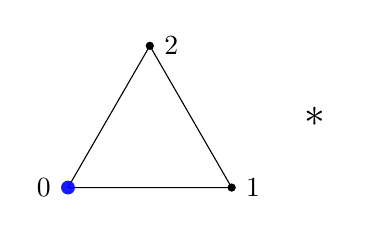
\begin{tikzpicture}[scale=.6]
\coordinate (A) at (210:2);
\coordinate (B) at (-30:2);
\coordinate (C) at (90:2);

\draw[draw=black] (A) -- (B) -- (C) -- (A);

\node[circle,fill=blue, opacity=.9, inner sep=0pt,minimum size=5pt, label=left:{0}] (a) at (A) {};
\node[circle,fill=black,inner sep=0pt,minimum size=3pt, label=right:{$1$}] (a) at (B) {};
\node[circle,fill=black,inner sep=0pt,minimum size=3pt, label=right:{$2$}] (a) at (C) {};

\node[scale=1.5] at (3.5,0.5) {$\ast$};
\end{tikzpicture}
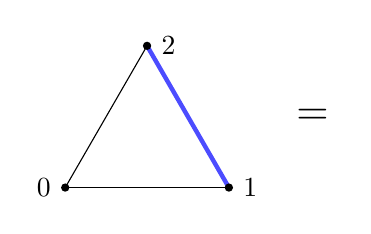
\begin{tikzpicture}[scale=.6]
\coordinate (A) at (210:2);
\coordinate (B) at (-30:2);
\coordinate (C) at (90:2);

\draw[draw=blue, ultra thick, draw opacity=.7] (B) -- (C);
\draw[draw=black] (C) -- (A);
\draw[draw=black] (A) -- (B);

\node[circle,fill=black,inner sep=0pt,minimum size=3pt, label=left:{$0$}] (a) at (A) {};
\node[circle,fill=black,inner sep=0pt,minimum size=3pt, label=right:{$1$}] (a) at (B) {};
\node[circle,fill=black,inner sep=0pt,minimum size=3pt, label=right:{$2$}] (a) at (C) {};

\node[scale=1.5] at (3.5,.5) {=};
\end{tikzpicture}
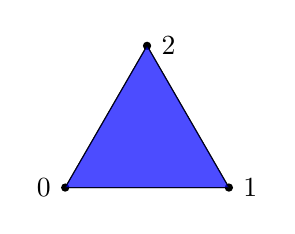
\begin{tikzpicture}[scale=.6]
\coordinate (A) at (210:2);
\coordinate (B) at (-30:2);
\coordinate (C) at (90:2);

\draw[draw=black] (A) -- (B) -- (C) -- (A);

\node[circle,fill=black,inner sep=0pt,minimum size=3pt, label=left:{$0$}] (a) at (A) {};
\node[circle,fill=black,inner sep=0pt,minimum size=3pt, label=right:{$1$}] (a) at (B) {};
\node[circle,fill=black,inner sep=0pt,minimum size=3pt, label=right:{$2$}] (a) at (C) {};

\draw[draw, fill=blue, opacity=.7] (A) -- (B) -- (C) -- (A);
\end{tikzpicture}
	\caption{Geometric representation of the join product of two basis elements. It depicts the identity $\big([0] \pr [1,2]\big) = [0,1,2]$.}
	\label{f:join of faces}
\end{figure}

The counital coalgebra structure on the tensor product of two $\cM$-bialgebras $C$ and $C'$ can be naturally extended to an $\cM$-bialgebra structure using
\[
(C \ot C^\prime) \ot (C \ot C^\prime) \xra{(23)}
C \ot C \ot C^\prime \ot C^\prime
\xra{\ \aug \ot \, \id \, \ot \, \pr + \pr \ot \, \id \, \ot \,\aug\ }
C \ot C^\prime.
\]

From these constructions we obtain a natural $\cM$-bialgebra structure, and, consequently a natural $E_\infty$-coalgebra structure, on each $\chains \big( \simplex^{n_1, \dots, n_k} \big) = \chains(\simplex^{n_1}) \ot \dotsb \ot \chains(\simplex^{n_k})$.
We can then extend these natural $E_\infty$-coalgebras to the chains on any multisimplicial set $X$.
Explicitly, \todo{@anibal: finish this}

We remark that, since the category of $\cM$-bialgebras is not cocomplete, we do not necessarily have an $\cM$-bialgebra structure on $\chains(X)$ for a general multisimplicial set $X$.
An example for which such structure does not exist is given by one such $X$ whose geometric realization consists of just two points.

\subsection{Steenrod cup-$(p,i)$ coproducts} \label{ss:cup coproducts}

In \cite{steenrod1947products}, Steenrod introduced natural operations on the mod~2 cohomology of spaces, the celebrated \textit{Steenrod squares}
\[
\begin{tikzcd} [column sep=small, row sep=0]
	\Sq^k \colon &[-20] \rH^{-n} \arrow[r] & \rH^{-n-k} \\ &
	{[\alpha]} \arrow[r, mapsto] & \big[ (\alpha \ot \alpha) \Delta_{n-k} \big],
\end{tikzcd}
\]
via an explicit construction of natural linear maps $\Delta_i \colon \chains(X) \to \chains(X) \ot \chains(X)$ for any simplicial set $X$, satisfying up to signs the following homological relations
\begin{equation} \label{e:cupi homological relations}
	\bd \circ \, \Delta_i + \Delta_i \circ \bd =
	(1 + T) \Delta_{i-1},
\end{equation}
with the convention $\Delta_{-1} = 0$.
These so-called \textit{cup-$i$ coproducts} appear to be fundamental.
%We mention two results supporting this claim.
%In higher category theory they define the nerve of $n$-categories \cite{medina2020globular} as introduced by Street \cite{street1987orientals}; and, in connection with K- and L-theory, the Ranicki--Weiss assembly \cite{ranicki1990assembly} can be used to show that chain complex valued presheaves over a simplicial complex $X$ can be fully faithfully modeled by comodules over the symmetric coalgebra structure they define on $\chains(X)$ \cite{medina2022assembly}.

%In the cubical case, cup-$i$ coproducts were defined in \cite{kadeishvili1999coproducts} and \cite{pilarczyk2016cubical}.
%The formulas used by these authors are similar to those introduced in \cite{medina2023fast_sq} for the simplicial case, a dual yet equivalent version of Steenrod's original.
A description of cup-$i$ coproducts for multisimplicial sets can be deduced from our $E_\infty$-structure:
%We first present it in a recursive form
\begin{equation} \label{e:recursive cup-i}
	\begin{split}
		& \Delta_0 = \Delta, \\
		& \Delta_i =
		(\ast \ot \id) \circ (23)(\Delta_{i-1} \ot \id) \circ \Delta.
	\end{split}
\end{equation}
A closed form formula for $\Delta_i$ is presented in \cite[\S4.8]{medina2021cube_einfty} for cubical chains.
The same formula, appropriately interpreted, holds for multisimplicial chains, which are their generalization.

%It is not known if the cup-$i$ coproducts defined in \cref{e:closed cup-i} agree with those previously constructed, for which a comparison is also missing.
%This highlights the value of a potential axiomatic characterization of cubical cup-$i$ coproducts as it exists in the simplicial case \cite{medina2022axiomatic}.
%
%As already mentioned, cup-$i$ coproducts represent the Steenrod squares at the chain level,
%which are primary operations in mod~2 cohomology.
%To obtain secondary cohomology operations one studies the cohomological relations these operations satisfy, for example the Cartan and Adem relations \cite{steenrod1962cohomology}.
%To do this at the cubical cochain level, as it was done in \cite{medina2020cartan,medina2021adem} for the simplicial case, the operadic viewpoint is important, so our $E_\infty$-structure on cubical cochains invites the construction of cochain representatives for secondary operations in the cubical case.

For $p$ an odd prime, Steenrod also introduced operations on the mod~$p$ cohomology of spaces using the homology of symmetric groups \cite{steenrod1952reduced, steenrod1953cyclic}.
Using the operadic framework of May \cite{may1970general}, we described in \cite{medina2021may_st}
%elements in $\UM$ representing
multicooperations defining Steenrod operations at any prime for certain $E_\infty$-coalgebras.
In particular, these so-called \textit{cup-$(p,i)$ coproducts} are defined, after the present work, on multisimplicial chains using $\copr$, the permutations of factors, and $\pr$.
%The aforementioned construction of cubical cup-$(p,i)$ coproducts has been implemented in the open source computer algebra system \href{https://comch.readthedocs.io/en/latest/}{\texttt{ComCH}} \cite{medina2021comch}.
